
\subsection*{Running only MPI or openMP}



\subsection*{How many nodes is best}

\subsection*{Hybrid vs pure distributed memory model}

To test the hybrid and the pure distributed memory model we do a few runs on Kongull with the following settings such that $n = 16384$,  $t\cdot p = 36$ and $p = \{1, 2, 3, 4, 6, 9, 12, 18, 36\}$.
\begin{figure}
\centering
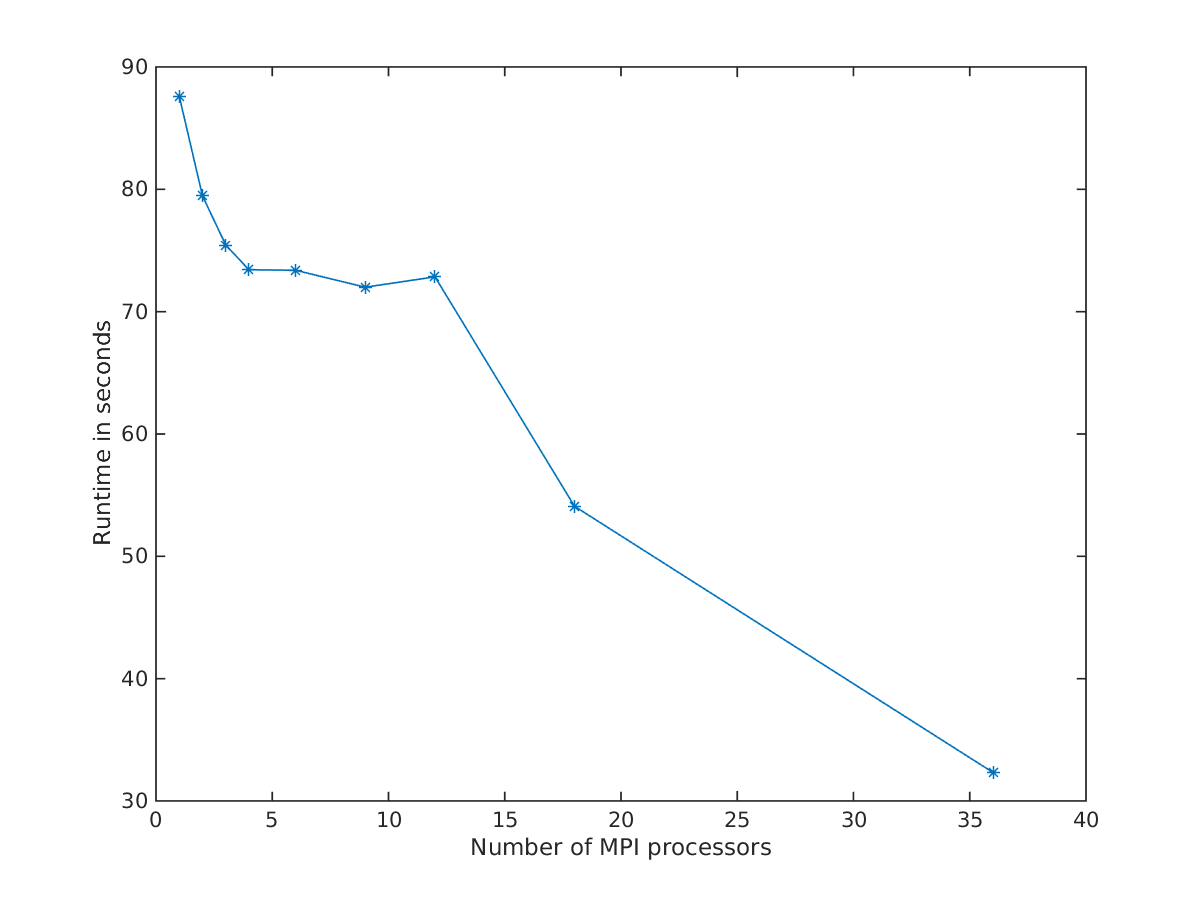
\includegraphics[width=0.7\textwidth]{./figures/runtime}
\caption{Runtime with different numbers for MPI processors and openMP threads with $p\cdot t = 36$.}
\label{fig:runtime}
\end{figure}
As seen in figure \ref{fig:runtime} the pure distributed model outclasses the hybrid model. This may be the case since the problem is pretty local in the sense that we don't need many MPI calls. We need, however, quite a few openMP calls. It seems reasonable that for this problem the pure distributed memory model works best since we only need to send data between nodes twice, and it may be most efficient to just spread the data all the way from the beginning. More testing shows that even when just using one node (and twelve cores) the pure distributed model performs better than the hybrid model.


\subsection*{Speedup and parallel efficiency}
Inspired by that was discovered in the last section we now focus on speedup and efficiency only on the pure distributed model.
\begin{figure}
        \centering
        \begin{subfigure}[b]{0.45\textwidth}
			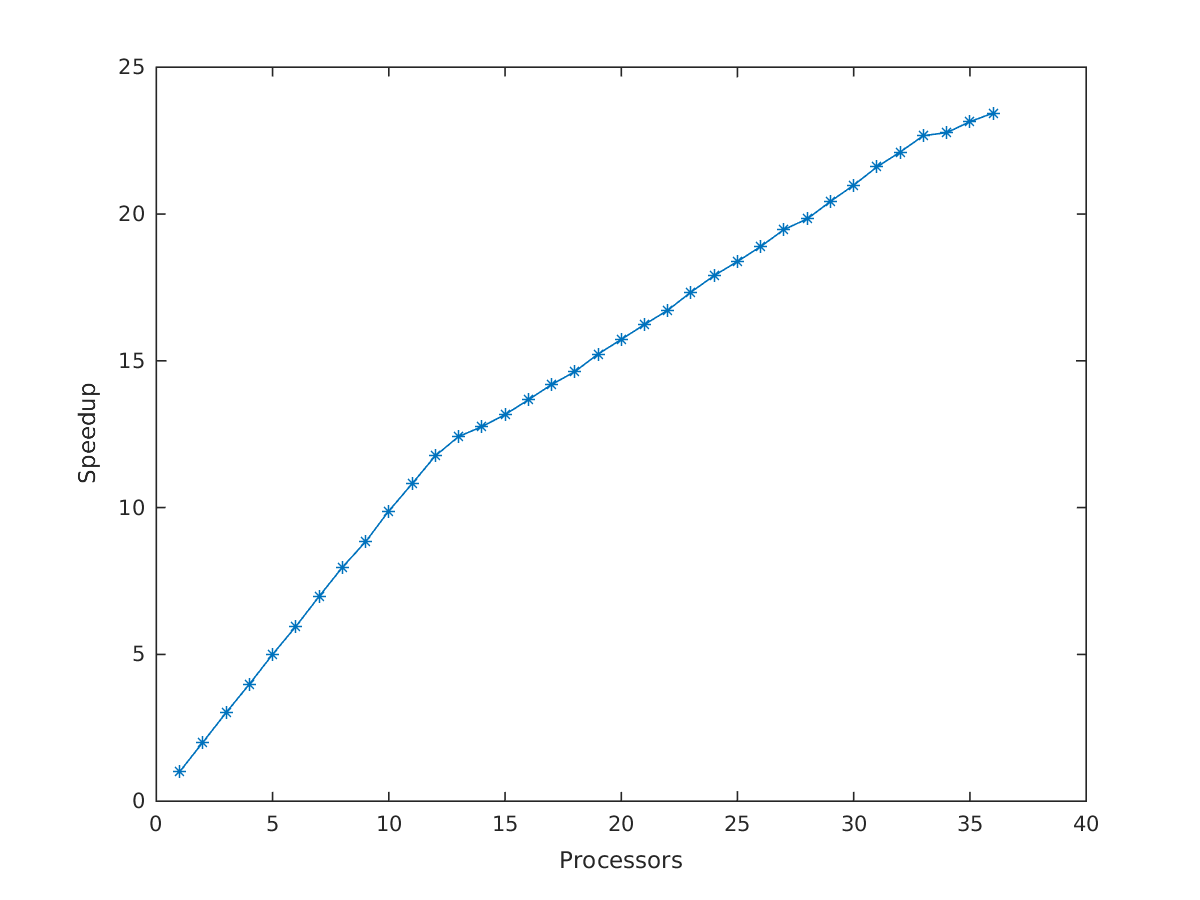
\includegraphics[width=\textwidth]{./figures/speedup}
			\caption{Parallel speedup.}
			\label{fig:speedup}
        \end{subfigure}
        ~ %add desired spacing between images, e. g. ~, \quad, \qquad, \hfill etc.
          %(or a blank line to force the subfigure onto a new line)
        \begin{subfigure}[b]{0.45\textwidth}
			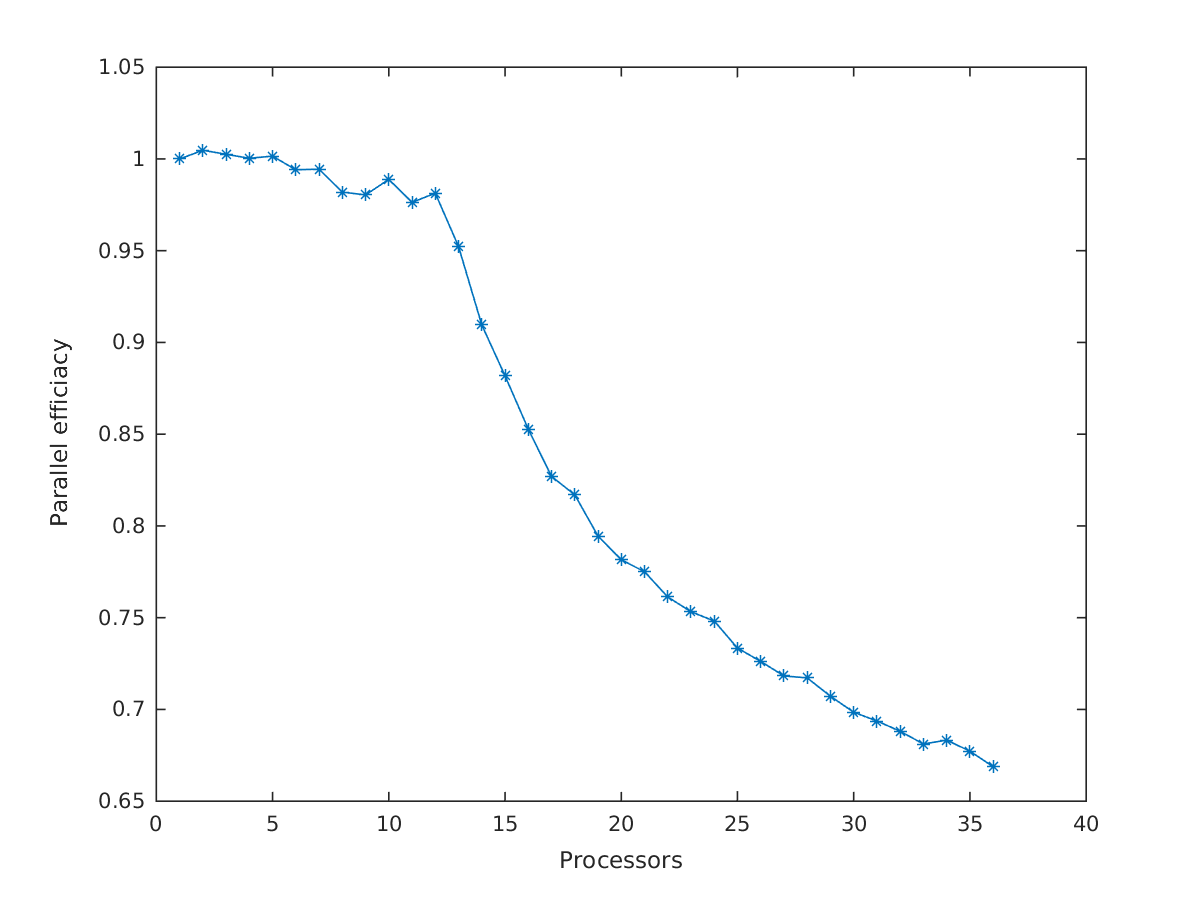
\includegraphics[width=\textwidth]{./figures/efficiacy}
			\caption{Parallel efficiency.}
			\label{fig:efficiacy}
        \end{subfigure}%
        \caption{Parallel speedup and efficiency for the pure distributed memory model}
        \label{fig:analysis}
\end{figure}

As can be seen in figures \ref{fig:speedup} and \ref{fig:efficiacy} we get a really good speedup and the parallel efficiency is almost ideal as long we only use a single node with 12 processors. With more than 12 processors the efficiency drops, but the speedup still makes it worth it. We assume this happens because the network overhead of using more than one node inhibits the efficiency more than the overhead of transporting things inside the node itself.


\subsection*{How does runtime scale with N}